\begin{figure}[t]
\centering
 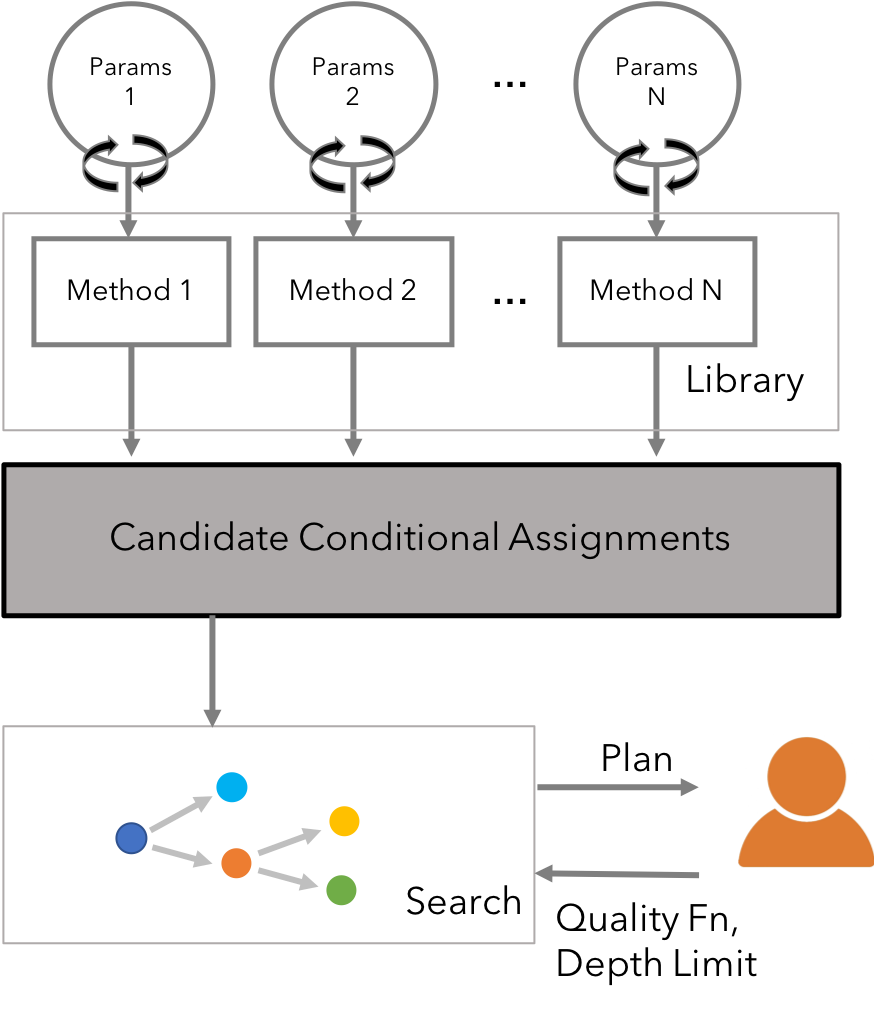
\includegraphics[width=0.7\columnwidth]{figures/architecture.png}
 \caption{\small \sys decouples sampling from the parameter space from search. This allows the user to iterate quickly by observing early best-effort results. \label{fig:arch}}
\end{figure}



\section{Approach Outline}

\sys takes as input a user-provided quality function $Q$, and searches through the space of candidate pipelines $\mathcal{P}$ to find a cleaning pipeline $p*\in\mathcal{P}$ that maximizes the resulting quality of the relation $Q(p*(R))$.  \sys is progressive: at any time, \sys reports the best cleaning pipeline found so far.  This helps the user trade-off between search time and cleaning quality.

Recall that a pipeline is composed of conditional assignments, which are generated by executing cleaning operators with specific parameter values.   A naive approach would select an operator $o$, draw a sample $\phi$ from its parameter space, execute $o(\phi)$ to generate a set of conditional assignments.  It then composes each conditional assignment $ca_i$ to each pipeline $p_j$ in the current pool of candidates, execute the new pipeline $p' = ca_i \circ p$, and evaluate the quality function $Q(p'(R))$.

% Each conditional assignment can be appended to the current pool of candidate pipelines,  and then extend the current pool of candidate pipelines with the new condi  Thus the cost to execute a given cleaning operator can be an enormous bottleneck on the ability to generate candidate pipelines.  

%The space of possible conditional assignments and cleaning pipelines is far too large, and only a small subset is feasible to materialize at any time. 

This section describes a naive approach that we call {\it Synchronous Tuning}, and the architectural decisions to enable progressive pipeline generation.


\subsection{Synchronous Tuning}

A naive approach plan enumeration is straightforward.  To generate the next candidate pipeline, select a candidate cleaning operator, select parameter values and execute the operator to generate a set of candidate assignments, select one candidate assignment and select a predicate for it, append it to the current candidate pipelines, and finally evaluate the quality function.  In fact, many existing data cleaning systems~\cite{} implicitly use this search procedure, but avoid the large branching factor through careful system design.    However, each step to generate a new candidate pipelines is blocking, and considerably slows the ability to quickly search through candidate pipelines.  

To address this issue, we explicitly decouple the generation of candidate assignments from the search procedure.  \sys .  In a parallel procedure, 

This paper proposes a framework, called \sys, that provides a simple unified abstraction of cleaning transformations and facilitates optimization over a plan space of cleaning transformation sequences.
We now describe how \sys enumerates the plan space.

\subsection{Candidate Conditional Assignment Set}
Our main architectural insight is a generate-then-search framework.
Possible parameter values are fed into a library of data cleaning methods, and these parameter assignments asynchronously generate candidate repairs to the dataset (called conditional assignments).
In parallel, a search thread builds a data cleaning plan using compositions of those transformations in the set. 
Existing search algorithms implicitly pipeline these two steps; whereas, we decouple these two steps where candidate repairs can be generated in a separate thread and the search algorithm can proceed independently.
This contrasts from the baseline architecture, hereafter called \emph{synchronous tuning}, where a hyperparameter tuning algorithm will then select and assign parameter values to a sequence of operators and evaluate the quality at the end. 
There are a few benefits for the asynchronous architecture of \sys.

\vspace{0.5em} \noindent \textbf{Benefit 1. Robustness To Straggler Data Cleaning Methods: } Decoupling candidate generation and search allows \sys to be robust to particular data cleaning methods that are slow. Many data cleaning methods have parameters that affect their runtime. For example, inference thresholds and partitioning parameters can have ``cliffs'', where a small change in parameters can drastically slow down the performance of the method. Including such parameter settings in the search process naively would block the entire system.

\vspace{0.5em} \noindent \textbf{Benefit 2. Progressive Results: } Next, the decoupling also allows for improved progressive behavior with early results. The search thread continuously polls the candidate conditional assignment set for new expansions. The naturally faster  data cleaning methods (e.g., approximate) will generate candidate repairs faster. Slower methods will eventually add these candidate repairs. This allows users to identify faults or glitches in their quality specifications or parameter spaces more quickly than if all methods were synchronously tuned in a pipeline.

\subsection{Parameter Space}
The input parameters to each of the data cleaning methods follow a type system that allows us to apply some optimizations based on the quality function.

\noindent \textbf{General Parameters: } \sys also accepts lists of general parameters, which can any python object. The user must specify the list of possible values and no optimizations can be applied to prune this space.

\noindent \textbf{Attribute Name Parameters: } These are parameter with an attribute name (or multiple attributes) as a property. For example, a numerical outlier detection algorithm might apply to a single attribute or a subset of attributes. The search space over possible attribute names is automatically generated from the schema. \sys ``pushes up'' the attributes relevant to the quality function to eliminate generating candidates for irrelevant attributes. 

\noindent \textbf{Numerical Parameters: } Another broad class of parameters in data cleaning methods are numerical parameters like thresholds and inference parameters. For these parameters, the user specifies a range (or a multi-dimensional grid). Often times, these parameters correspond to confidence metrics. In the example with the \texttt{City} table, the \texttt{ispell} method has a acceptance threshold for spell-checking. In these cases, we recommend that this search space is ordered fine-to-coarse. Where the most restrictive threshold is evaluated first towards increasingly less restrictive thresholds. 

\subsection{Incremental Evaluation}
The main drawback of the asychronous approach is that the number of quality function evaluations is much higher. We argue that this is acceptable in many data cleaning settings, since quality function evaluation is often far cheaper than candidate repair generation (e.g., checking integrity constraints is cheaper than enforcing them). Furthermore, \sys can ``incrementally'' evaluate a quality function. 
Suppose we have a relation $R$, the quality function $q$, and a set of conditional assignment expressions $C$.
When possible, \sys computes $q(R)$ once and then for each of the expressions $c \in C$ compute a delta $q(c(R)) = q(R) + \delta_c(q(R))$.
For many types of quality functions such incremental computation can be automatically synthesized and can greatly save on computation time.
This is exactly a process of incremental view maintenance.

Let us consider a concrete example with the quality function q1, a functional dependency checker, from the previous section.
$R'$ is the resulting relation after applying \texttt{c} to all of the records.
Let $r_{pred}$ be the set of records that satisfy the predicate of the conditional assignment expression and $r_{pred}'$ be the resulting transformed records.
q1 can be expressed in relational algebra in the following way:
\[
q_1(R') = \textsf{count}( R' \bowtie R' )
\]
$R'$ can be described in terms of $R$:
\[
R' = R - r_{pred} + r_{pred}' 
\]
leading to the following expression:
\[
q_1(R') = \red{q_1(R)} - \textsf{count}( r_{pred} \bowtie R )  + \textsf{count}( r'_{pred} \bowtie R )
\]
If we used a hash join to evaluate this quality function, the cost of incrementally maintaining is roughly linear in the size of the number records changed rather than the size of the relation.

The consequence is that evaluating changes in quality can be very efficient for a large class of data cleaning problems.
The architecture of \sys is designed to exploit this property.
We assume conditional assignment generation to be expensive but quality evaluation to be fast.
An architecture that runs the entire pipeline before seeing the resultant quality is wasteful.




